\section{録音した音声の操作}
本課題を行うにあたって大事なことを説明する。
\begin{itemize}
\item サンプリング周波数Fsとは、「1秒間に処理できるデータの数」のことである。
\item 「波形の上下を反転する」とは、データの各要素を-1倍することに等しい。
\item 「データ数」「要素数」はそれぞれ取得できる関数が存在する。
\end{itemize}

\subsection{上下反転スクリプト}
上でも説明したように、各要素を-1倍してやれば良い。よってfor文を用いて記述可能である。行列から指定した要素をとってきて、それを-1倍することを要素の個数分繰り返してやれば良い。以下にヒントを示す。\footnote{実際には変換前と変換後のデータが必要なことに注意}\footnote{yと同じサイズの行列を用意すれば…?}
\begin{verbatim}
for k=1:N;
    y(○)=y(○)*○;
end
\end{verbatim}

\subsection{成功例}
\begin{figure}[H]
  \begin{minipage}{0.45\linewidth}
    \centering
    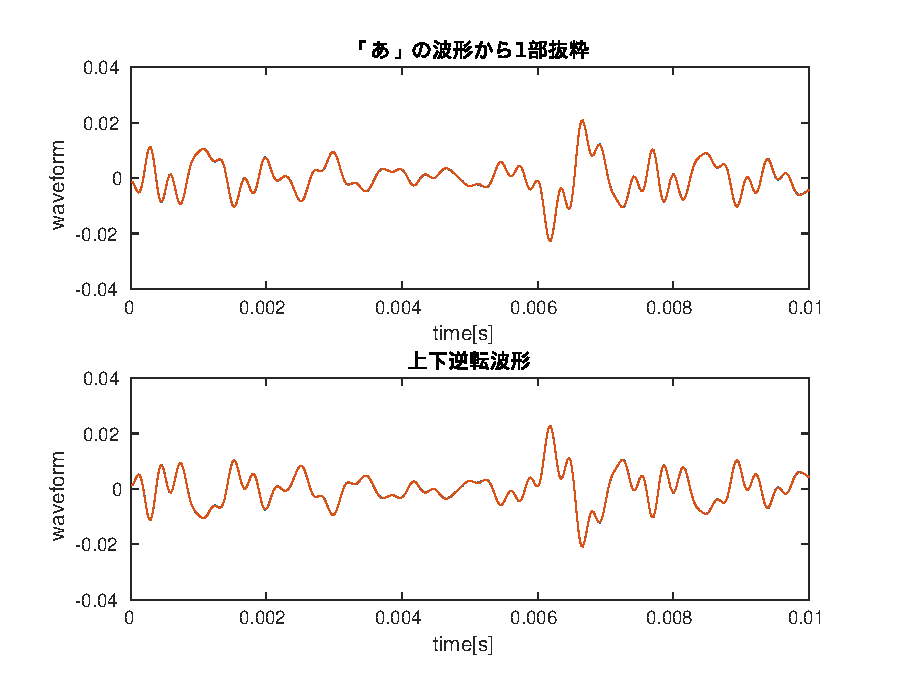
\includegraphics[scale=0.5]{../eps/kadai2_a.eps}
  \end{minipage}
  \begin{minipage}{0.45\linewidth}
    \centering
    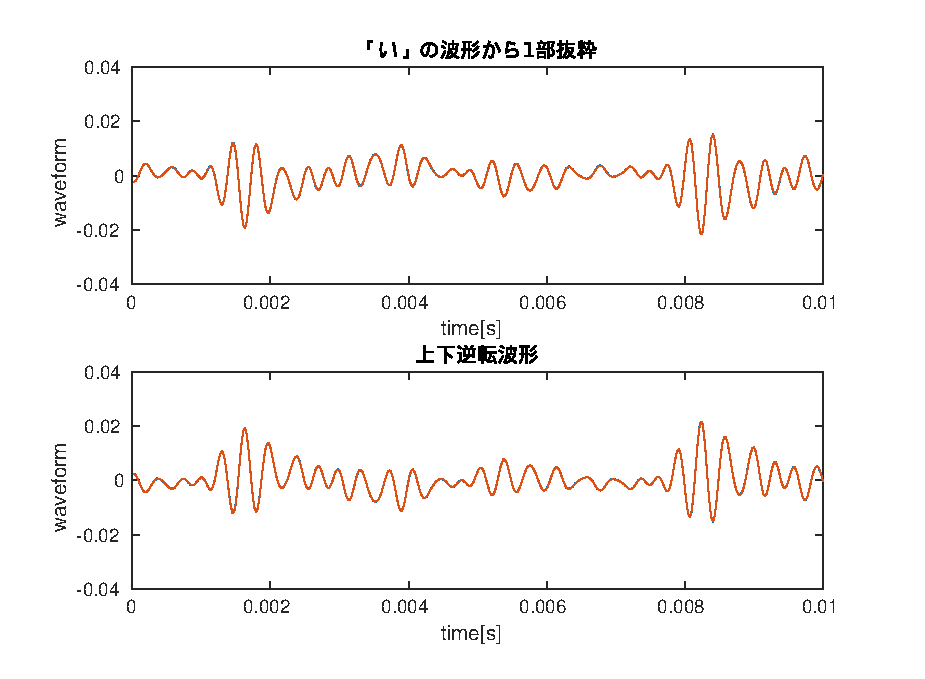
\includegraphics[scale=0.5]{../eps/kadai2_i.eps}
  \end{minipage}
\end{figure}

\end{document}
